\newpage
{\bfseries IRSTI 65.33.91}
\hfill {\bfseries \href{https://doi.org/10.58805/kazutb.v.2.23-373}{https://doi.org/10.58805/kazutb.v.2.23-373}}

\sectionwithauthors{M.Zh. Yessembek, B.K. Tarabayev, A.M. Omaraliyeva}{INCREASING OF MICROBIOLOGICAL STABILITY OF BREAD WITH USING
SECONDARY RAW MATERIALS FROM CEREAL PROCESSING}

\begin{center}
{\bfseries \textsuperscript{1}M.Zh. Yessembek\envelope, B.K. Tarabayev\textsuperscript{1}, \textsuperscript{2}A.M. Omaraliyeva}

\textsuperscript{1}NCJSC S.Seifullin Kazakh Agro Technical Research
University, Astana, Kazakhstan,

\textsuperscript{2}JSC Kazakh University of Technology and Business
named after K. Kulazhanov, Astana, Kazakhstan,

\envelope Corresponding author: aygerim\_talgatqyzy@mail.ru
\end{center}

Bread and bakery products are one of the main food products, and their
quality does not always meet the requirements of modern nutrition
science. One of the directions of solving this problem is the creation
of new safe varieties of bakery products of functional purpose to
correct the nutrition of the population. The article considers the
causes of microbial spoilage, the negative influence of mold fungi and
spore-forming bacteria of the genus \emph{Bacillus} on the safety of
bread with the use of secondary raw materials of grain crops processing.
The main objects of research were bakery products with the use of rice
and buckwheat brans, prepared by the traditional method and on complex
sourdough starter. Studies on the influence of the method of rice and
buckwheat brans application on resistance to mold and potato disease
infection were conducted.

{\bfseries Keywords:} Microbiological safety, bread, secondary raw
materials, rice bran, buckwheat bran, fermented brew, mold, potato
disease.

\begin{center}
{\large\bfseries ДӘНДІ ДАҚЫЛДАРДЫ ҚАЙТА ӨҢДЕУДІҢ ЕКІНШІЛІК ШИКІЗАТЫН ҚОЛДАНА
ОТЫРЫП НАННЫҢ МИКРОБИОЛОГИЯЛЫҚ ТҰРАҚТЫЛЫҒЫН АРТТЫРУ}

{\bfseries \textsuperscript{1}М.Ж. Есембек\envelope, \textsuperscript{1}Б.К. Тарабаев, \textsuperscript{2}А.М. Омаралиева}

\textsuperscript{1} С.Сейфуллин атындағы Қазақ агротехникалық зерттеу
университеті» КеАҚ,

Астана, Қазақстан,

\textsuperscript{2}Қ. Құлажанов атындағы Қазақ технология және бизнес
университеті АҚ,

Астана, Қазақстан

e-mail: yessembek.madina@gmail.com
\end{center}

Нан және нан өнімдері негізгі тағамдардың бірі болып табылады және
олардың сапасы қазіргі заманғы тамақтану ғылымының талаптарына әрдайым
сәйкес келе бермейді. Бұл мәселені шешудің бір бағыты -- халықтың
тамақтануын түзету үшін функционалды мақсаттағы нан өнімдерінің жаңа
қауіпсіз сорттарын әзірлеу. Мақалада дәнді дақылдарды қайта өңдеудің
екіншілік шикізатын қолдана отырып нанның қауіпсіздігіне микробтардың
бүліну себептері, зең саңырауқұлақтары мен \emph{Bacillus} тектес спора
түзетін бактериялардың кері әсері қарастырылады. Негізгі зерттеу
нысандары дәстүрлі әдіспен және кешенді ашытқымен дайындалған күріш және
қарақұмық ұншығынан жасалған нан өнімдері болды. Күріш және қарақұмық
ұншығын енгізу әдісінің көгеруге және картоп ауруына төзімділігіне әсері
бойынша зерттеулер жүргізілді.

{\bfseries Түйін сөздер:} Микробиологиялық қауіпсіздік, нан, екіншілік
шикізат, күріш ұншығы, қарақұмық ұншығы, ашытылған қайнатпа, көгеру,
картоп ауруы.

\begin{center}
{\large\bfseries ПОВЫШЕНИЕ МИКРОБИОЛОГИЧЕСКОЙ УСТОЙЧИВОСТИ ХЛЕБА С ПРИМЕНЕНИЕМ
ВТОРИЧНОГО СЫРЬЯ ПЕРЕРАБОТКИ ЗЕРНОВЫХ КУЛЬТУР}

{\bfseries \textsuperscript{1}М.Ж. Есембек\envelope, \textsuperscript{1}Б.К. Тарабаев, \textsuperscript{2}А.М. Омаралиева}

\textsuperscript{1}НАО «Казахский агротехнический исследовательский
университет им. С.Сейфуллина, Астана, Казахстан,

\textsuperscript{2}АО Казахский университет технологии и бизнеса им.К.
Кулажанова,

Астана, Казахстан

e-mail: yessembek.madina@gmail.com
\end{center}

Хлеб и хлебобулочные изделия являются одним из основных продуктов
питания, а их качество далеко не всегда соответствует предъявляемым
требованиям современной науки о питании. Одним из направлений решения
данной проблемы является создание новых безопасных сортов хлебобулочных
изделий функционального назначения для коррекции питания населения. В
статье рассмотрены причины микробной порчи, отрицательное влияние
плесневых грибов и спорообразующих бактерий рода \emph{Bacillus} на
безопасность хлеба с применением вторичного сырья переработки зерновых
культур. Основными объектами исследований выступали хлебобулочные
изделия с использованием рисовой и гречневой мучек, приготовленные
традиционным способом и на комплексной закваске. Проведены исследования
по влиянию способа внесения рисовой и гречневой мучек на устойчивость к
плесневению и заражению картофельной болезнью.

{\bfseries Ключевые слова:} Микробиологическая безопасность, хлеб,
вторичное сырье, рисовая мучка, гречневая мучка, заквашенная заварка,
плесневение, картофельная болезнь.

\begin{multicols}{2}
{\bfseries Introduction.} In the modern world food production is put on a
stream, a stable process of production of high-quality bakery products
is impossible without the purposeful use of food additives, improvers,
various types of raw materials. They have a wide functional range, have
the properties to affect the components of raw materials, give a certain
quality to finished products, increase nutritional value, and also give
the opportunity to form certain properties of dough from flour with
unstable baking characteristics.

Ingredients, with the help of which it is possible to increase the
nutritional value of wheat bread, are currently very diverse. The most
appropriate is the use of non-traditional ingredients of plant origin,
containing a high amount of proteins, micro and macronutrients. When
they are used, the therapeutic and preventive value of wheat bread
increases {[}1, 2{]}. One of such ingredients is rice and buckwheat bran
{[}3{]}. These raw materials contain a wide range of biologically active
substances, which, when added to food, have a beneficial effect on the
human body.

Analysis of scientific and industrial developments indicate that there
are numerous studies on the use of secondary raw materials of cereal
crops for enrichment of bakery products. However, currently a serious
problem of bakery products is their vulnerability to microbial spoilage
under the action of bacteria and mold fungi, as it not only leads to
deterioration of the appearance of bakery products, but also negatively
affects their quality and safety.

The most dangerous and widespread disease of bread is considered to be
potato disease, which is often observed in regions with hot climate and
in summer time. In recent years, due to the widespread use of packaging
in polymeric materials, which is a provoking factor for the development
of microbial spoilage, the spread of cases of potato disease is noted
not only in the southern regions, but also in the northern regions of
Kazakhstan and in the spring-summer period, and in winter {[}4, 5{]}.
The causative agents of this disease are spore-forming bacteria of the
genus \emph{Bacillus}. Spores of potato bread disease pathogens, unlike
mold fungi, are able to persist in the finished product after baking.

Affected bread first loses its natural taste and aroma, then a peculiar
sweetish odor appears in it, which as the disease develops intensifies
and the smell of bread acquires a rotten tinge. Under the influence of
active enzymes of the causative agent of potato bread disease, there are
significant changes in the structure of the bread crumb: dark smearing
and pulling threads appear inside.

The second common type of microbial spoilage of bakery products is mold,
which occurs as a result of the development of mold fungi of the genera
\emph{Aspergillus (А. fiavus, А. fumigatus, А. glaucus, А. nidulans, А.
niger, А. ochaceus), Mucor (М. mucedo, М. pusillus, М. spinosus),
Penicillium (Р. crustosum, Р. expansum), Rhizopusnigricans,
Geotrichumcandidum.} The surface of bread affected by mold is covered
with fluffy plaque of various colors: gray, white, green, yellow,
bluish, black {[}6{]}. The bread comes out of the oven sterile, i.e.
mold is a secondary contamination.

Mould fungi adversely affect the quality of raw materials and finished
bread. They cause profound changes in bread by breaking down proteins,
carbohydrates and fats with the help of their enzymes. Bread that is
affected by mold fungi has an unpleasant taste and musty odor. About 80
species of mold fungi produce mycotoxins. Mycotoxins can cause health
problems in people who consume bread affected by mold fungi {[}7{]}.

A promising step in combating microbial spoilage of bread using
secondary raw materials of cereal crop processing is the use of
substances of natural origin that have a preserving effect, such as
metabolites of lactic acid bacteria, such as organic acids and
bacteriocins. The use of sourdough starters to inhibit microbial
spoilage of bread has been the subject of much research in recent years.
It is proved that bread prepared on sourdough starter with directed
cultivation is characterized by improved porosity structure and crumb
properties, taste and odor, microbiological purity, ability to preserve
freshness for a long time. The use of sourdough starter bred on pure
cultures of starter microorganisms allows to increase microbiological
safety and quality of bread.

In this regard, the research on the development of bread assortment with
the use of secondary raw materials of grain crops processing of improved
quality, increased nutritional value and microbiological stability is
relevant.

The purpose of the present research was to study the influence of the
method of rice and buckwheat brans application on the resistance of
bakery products to mold and potato disease development.

{\bfseries Materials and methods.} The research was carried out on the
basis of the ``Laboratory of innovative technologies and assortment of
bakery products'' of the St. Petersburg branch of the Federal State
Autonomous Scientific Institution ``Research Institute of Baking
Industry''. The objects of research were bakery products with the use of
rice and buckwheat brans, prepared by traditional method and on complex
sourdough starter. The control sample of bread was prepared without the
addition of rice and buckwheat brans by the method of trial laboratory
baking.

In the traditional method, 5\% rice bran and 10\% buckwheat bran in dry
form and 85\% first grade wheat flour, salt and pressed baking yeast,
sugar according to the recipe and water in the amount providing dough
moisture 48.0\% were added to the dough.

When preparing dough on complex sourdough starter, the sourdough starter
was prepared in accordance with the ``Collection of technological
instructions for the production of bakery products'' {[}8,9{]}, bred on
pure cultures of microorganisms in liquid form.

The peculiarity of the preparation of dough on complex sourdough starter
is the use of complex sourdough starter, by fermenting of sugared brew
at a temperature of 32-34°C. Also using a composition of pure cultures
of starter microorganisms. These compositions have probiotic properties
and antibiotic action against spore microflora. At the same time,
traditional biological starters (thick, liquid without brewing, liquid
with brewing) are excluded from the technological process, the amount of
flour introduced in brewed form (25-35\%) is increased.

Preparation of complex sourdough starter includes dilution and
production cycles.

For preparation of complex sourdough starter were used pure cultures of
lactic acid bacteria \emph{L.plantarum 1, L. brevis E120,} (1.5 ml each)
and yeast \emph{S.cerevisiae st. L-1} (1 ml of aqueous suspension).

The dilution cycle was used with a small mass of sourdough starter (500
g in the first phase). Microbial cultures were fused together, added to
the saccharified brew of rice and buckwheat brans with the addition of
unfermented barley malt (2\% to the weight of brans) and water, and left
to ferment for 20 hours.

The complex sourdough starter bred by breeding cycle using pure cultures
of lactic acid bacteria and starter yeast in liquid form in the
production cycle was maintained by refreshing with sugared brew in the
ratio of 1:1 - 1:9, i.e. complex sourdough starter - nutrition (sugared
brew) depending on the duration of sourdough starter fermentation.

80\% of the complex sourdough starter obtained was used for bread
production and the remaining part (20\%) was used for its refreshing.

To establish the influence of bread preparation technology on the rate
of mold development, we conducted model experiments with the infection
of its sterile slices with pure culture of mold fungi \emph{Penicillium
chrysogenum} {[}10,11{]}.

To determine the possibility of suppressing the potato disease of bread,
the method of putting finished products infected with spore bacteria
into conditions provoking the development of \emph{B. subtilis} was
used. To create provoking conditions, dry bread crumbs infected with
\emph{B. subtilis} spore-forming bacteria and containing
10\textsuperscript{8} KOE/g of spores were introduced during dough
kneading. To determine the content of \emph{B. subtilis} spores in the
infected crumb, the method described in the book ``Microbiology of
Baking Production'' (Afanasyeva O.V., 2003) was used {[}12{]}. Bread was
stored according to the Instruction for the prevention of potato bread
disease {[}13{]}, for which immediately after baking the bread was
wrapped in damp paper and placed in a thermostat at 37°C. After 24
hours, the bread was cut with a knife and the presence of signs of
disease (specific unpleasant odor, sticky crumb) was determined
visually. In the absence of the disease, the bread was further incubated
under the same conditions.

{\bfseries Results and discussion.} In the preparation of bread using rice
and buckwheat brans by the traditional method, it was found that the use
of secondary raw materials in dry form provokes the growth of mold fungi
during the storage of bread compared to products prepared on complex
sourdough starter and without the addition of secondary raw materials.

At infection of sterile bread slices with rice and buckwheat brans on
complex sourdough starter, pure culture of mold \emph{Penicillium
chrysogenum}, mold spores did not appear, which proves that the use of
secondary raw materials in the form of fermented brew during dough
kneading provides its microbiological purity, especially resistance of
bread to mold. At the same time on the surface of bread slices prepared
with rice and buckwheat brans in dry form, mold growth was observed
after 26 hours. While on a slice of control bread, prepared from
first-grade wheat flour without the addition of secondary raw materials,
mold spores appeared after 28 hours (Fig. 1).
\end{multicols}

\begin{figure}[H]
	\centering
	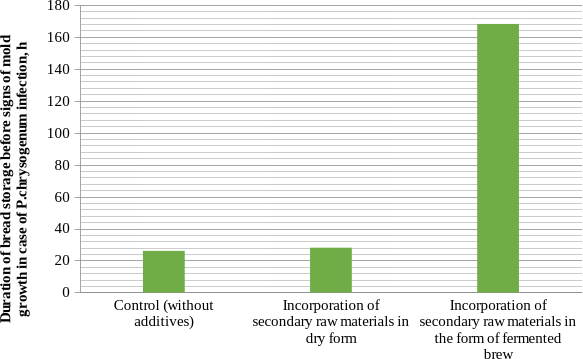
\includegraphics[width=0.6\textwidth]{assets/1108}
    \caption*{Figure 1 - Effect of rice and buckwheat brans application method on bread resistance to moldiness}
\end{figure}

\begin{figure}[H]
	\centering
	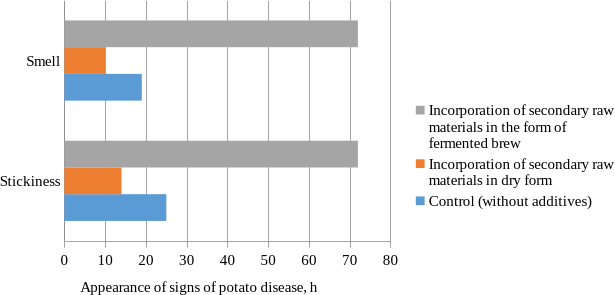
\includegraphics[width=0.7\textwidth]{assets/1109}
    \caption*{Figure 2 - Effect of rice and buckwheat brans application method on resistance to potato bread disease}
\end{figure}

\begin{multicols}{2}
Considering that the biological method involving the use of acidifying
components is one of the most effective ways to protect bread from
potato blight, the effect of rice and buckwheat brans on the suppression
of potato bacillus spores was investigated.

As a result of trial baking it was found that the appearance of signs of
potato disease after 10 hours in the form of unpleasant odor and after
14 hours - stickiness of the crumb, was observed in the sample of bread
prepared with the addition of rice and buckwheat brans in dry form. In
the control sample of bread prepared from first grade wheat flour
without the addition of secondary raw materials, unpleasant odor and
stickiness of the crumb appeared after 19 and 25 hours, respectively.
The bread sample with the addition of rice and buckwheat brans in the
form of fermented brew did not get potato disease (Fig. 2).

As a result of the conducted research it was found that the introduction
of rice and buckwheat brans in the form of fermented brew increases
antagonistic activity to \emph{Bacillus subtilis} and completely
suppresses the development of spores of potato bacillus.

{\bfseries Conclusions.} According to the results of studies of
microbiological indicators of bread quality it was found that the
application of secondary products of cereal crops: rice and buckwheat
brans in the form of fermented brew increases the resistance of bread to
mold and completely suppresses the development of potato disease. This
indicates that the introduction of secondary products of cereal crops in
the form of fermented brew has a significant effect on microbial
spoilage of bread, compared to traditional methods of bread preparation.
The results of the research can be recommended for use in the
development of multicomponent products based on secondary raw materials,
namely rice and buckwheat bran. This will improve the range of products
and diversify the nutrition of consumers seeking a healthy lifestyle.
\end{multicols}

\begin{center}
{\bfseries References}
\end{center}

\begin{noparindent}
1. Nikiforova T.A., Khon I.A., Baikov V.G. Ratsional\textquotesingle noe
ispol\textquotesingle zovanie vtorichnogo syr\textquotesingle ya
krupyanogo proizvodstva. // Khleboprodukty. -- 2014. - №6. -- S. 50-51.
{[}in Russian{]}

2. Nikiforova T.A., Khon I.A. Vliyanie grechnevoi muchki na sokhranenie
svezhesti khleba. // Khleboprodukty. - 2017. - №6. -- S.38-39. {[}in
Russian{]}

3. Esembek M.Zh., Tarabaev B.K., Omaralieva A.M., Botbaeva Zh.T.,
Kakimov M.M. Nan өndіrіsіnde paidalanu үshіn dәndі -- daқyldardy қaita
өңdeudің ekіnshіlіk shikіzatyn zertteu // Almaty tekhnologiyalyқ
universitetіnің khabarshysy. - 2022. - №1. - C. 29-35. DOI
10.48184/2304-568X-2022-1-29-35 {[}in Kazakh{]}

4. Dudikova D. Problemy kartofel\textquotesingle noi bolezni khleba v
Kazakhstane//Khleboprodukty. -- 2001. - № 11. -C. 23-26. {[}in
Russian{]}

5. Polyakova S.P. Metody i sredstva povysheniya mikrobiologicheskoi
bezopasnosti khlebobulochnykh izdelii // Khlebopechenie Rossii. - 2003.
- № 6. - S. 3-5. {[}in Russian{]}

6. Frolova Yu.M., Savkina O.A, Lokachuk M.N., Pavlovskaya E.N.,
Kuznetsova L.I., Parakhina O.I. Zakvaska kak sredstvo obespecheniya
mikrobiologicheskoi bezopasnosti khlebobulochnykh izdelii // Povyshenie
kachestva i bezopasnosti pishchevykh produktov: Materialy XII
Vserossiiskoi nauchno-prakticheskoi konferentsii s

mezhdunarodnym
uchastiem, posvyashchennoi 90-letiyu so dnya rozhdeniya doktora
tekhnicheskikh nauk, professora, Zasluzhennogo deyatelya nauki RF M.S.
Aminova, Makhachkala, 09--10 noyabrya 2022 goda. -- Makhachkala. --
2022. -- S. 110-112. {[}in Russian{]}

7. Dzh. M. Dzhei. Sovremennaya pishchevaya mikrobiologiya / Dzh. M.
Dzhei, M. Dzh. Messner, D. A. Gol\textquotesingle den.- M.: BINOM.
Laboratoriya znanii, 2017. --- 886 s. ISBN 978-5-9963-1300-6 {[}in
Russian{]}

8. Sbornik sovremennykh tekhnologii khlebobulochnykh izdelii / pod
obshchei redaktsiei chlen-korrespondenta Rossiiskoi akademii
sel\textquotesingle skokhozyaistvennykh nauk A. P. Kosovana. -- M. : GNU
GOSNII khlebopekarnoi

promyshlennosti, 2008. -- 268 s. {[}in Russian{]}

9. Pat. 7716 RK MPK A21D 8/02. Sposob prigotovleniya zakvaski dlya
proizvodstva khleba / M.Zh. Esembek, B.K. Tarabaev, L.I.Kuznetsova, A.M.
Omaralieva, Zh.T. Botbaeva. -№ 2022/0944.2; zayavl. 30.10.2022; opubl.
06.01.2023; Byul. №1. {[}in Russian{]}

10. Kuznetsova L.I, Savkina O.A., Ivanova E.S., Usova L.V., Ternovskoi
G.V. O plesnevenii khleba // Khlebopechenie Rossii. - 2014. - № 5. - S.
24-26. {[}in Russian{]}

11. Dubrovskaya N.O., Kuznetsova L.I., Savkina O.A. Vliyanie novoi
podkislyayushchei smesi na kachestvo rzhano-pshenichnogo khleba,
vyrabatyvaemogo po uskorennoi tekhnologii. // Khlebopechenie Rossii -
2014. - № 2. - S. 21-22. {[}in Russian{]}

12. Afanas\textquotesingle eva, O. V. Mikrobiologiya khlebopekarnogo
proizvodstva / O.V. Afanas\textquotesingle eva; S.-Peterb. fil. Gos.
nauch.-issled. in-ta khlebopekar. prom-sti (SPb F GosNIIKhP). - SPb. :
Beresta, 2003. - 220 s. {[}in Russian{]}

13. Instruktsiya po preduprezhdeniyu kartofel\textquotesingle noi
bolezni khleba na khlebopekarnykh predpriyatiyakh. -- M.: GNU GOSNIIKhP
Rossel\textquotesingle khozakademii, 2012. -- 32 s. {[}in Russian{]}
\end{noparindent}

\emph{{\bfseries Information about authors}}

\begin{noparindent}
Yessembek M.ZH. - Master of Technical sciences, NCJSC S.Seifullin Kazakh
Agro Technical Research University, Astana, Kazakhstan, e-mail:
yessembek.madina@gmail.com;

Tarabayev B.K. - Candidate of Technical Sciences, NCJSC S.Seifullin
Kazakh Agro Technical Research University, Astana, Kazakhstan, e-mail:
b.tarabayev@kazatu.edu.kz;

Omaraliyeva A.M. {\bfseries -} Candidate of Technical Sciences, JSC Kazakh
University of Technology and Business named after K. Kulazhanov, Astana,
Kazakhstan, e-mail: aigul-omar@mail.ru
\end{noparindent}

\emph{{\bfseries Авторлар туралы мәліметтер}}

\begin{noparindent}
Есембек М.Ж -- техника ғылымдарының магистрі, С.Сейфуллин атындағы Қазақ
агротехникалық зерттеу университеті КеАҚ, Астана, Қазақстан, e-mail:
yessembek.madina@gmail.com;

Б.К. Тарабаев - техника ғылымдарының кандидаты, «С.Сейфуллин атындағы
Қазақ агротехникалық зерттеу университеті КеАҚ, Астана қ., Қазақстан,
e-mail: b.tarabayev@kazatu.edu.kz;

Омаралиева А.М. - техника ғылымдарының кандидаты, Қ. Құлажанов атындағы
Қазақ технология және бизнес университеті АҚ, Астана, Қазақстан, e-mail:
aigul-omar@mail.ru
\end{noparindent}
